\section{Analysis and limitations}
\label{sec:analysis}

\begin{figure*}[t]
\centering
\setlength{\tabcolsep}{1.2pt}\renewcommand{\arraystretch}{0.6}
\begin{tabular}{@{}m{2.6cm}ccc@{}}
&\footnotesize\textbf{Original} & \footnotesize\textbf{Banksy} & \footnotesize\textbf{SteerVTE (ref.)} \\[2pt]
\scriptsize Correct original edited anyway; style lost & 
\includegraphics[width=0.27\linewidth]{figs/cells/fail_g043_en_glass_s1_orig.jpg} & 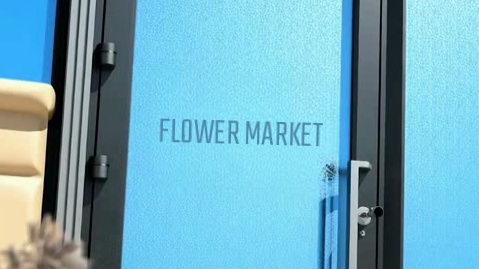
\includegraphics[width=0.27\linewidth]{figs/cells/fail_g043_en_glass_s1_B1.jpg} & 
\includegraphics[width=0.27\linewidth]{figs/cells/fail_g043_en_glass_s1_steervte.jpg} \\
&\parbox[t]{0.27\linewidth}{\centering\scriptsize \textcolor{okgreen}{\ding{51}}\,\texttt{FLOWER MARKET}} & \parbox[t]{0.27\linewidth}{\centering\scriptsize \textcolor{okgreen}{\ding{51}}\,\texttt{FLOWER MARKET}} & \parbox[t]{0.27\linewidth}{\centering\scriptsize \textcolor{okgreen}{\ding{51}}\,\texttt{FLOWER MARKET}} \\[3pt]
\scriptsize Erase patch, low contrast & 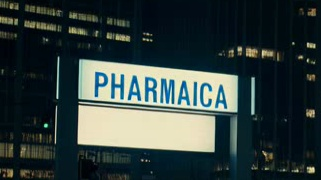
\includegraphics[width=0.27\linewidth]{figs/cells/fail_g026_en_signboard_s7_orig.jpg} & 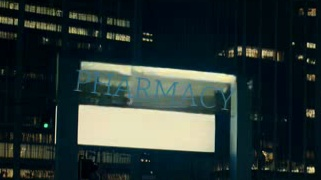
\includegraphics[width=0.27\linewidth]{figs/cells/fail_g026_en_signboard_s7_B1.jpg} & 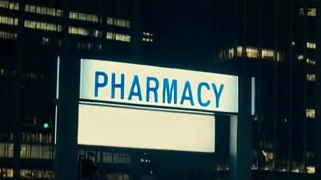
\includegraphics[width=0.27\linewidth]{figs/cells/fail_g026_en_signboard_s7_steervte.jpg} \\
&\parbox[t]{0.27\linewidth}{\centering\scriptsize \textcolor{badred}{\ding{55}}\,\texttt{PHARMAICA}} & \parbox[t]{0.27\linewidth}{\centering\scriptsize \textcolor{okgreen}{\ding{51}}\,\texttt{PHARMACY}} & \parbox[t]{0.27\linewidth}{\centering\scriptsize \textcolor{okgreen}{\ding{51}}\,\texttt{PHARMACY}} \\[3pt]
\scriptsize Outlined 3D letters flattened & 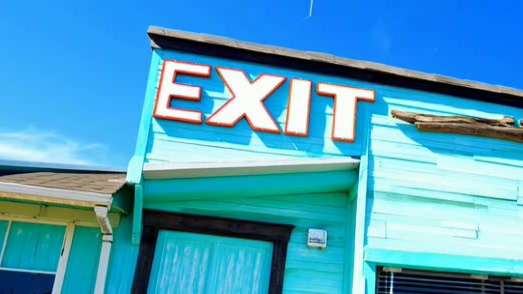
\includegraphics[width=0.27\linewidth]{figs/cells/fail_g014_en_wood_s3_orig.jpg} & 
\includegraphics[width=0.27\linewidth]{figs/cells/fail_g014_en_wood_s3_B1.jpg} & 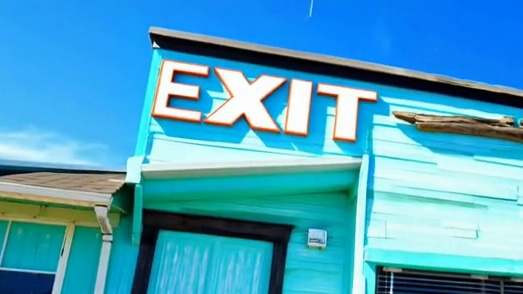
\includegraphics[width=0.27\linewidth]{figs/cells/fail_g014_en_wood_s3_steervte.jpg} \\
&\parbox[t]{0.27\linewidth}{\centering\scriptsize \textcolor{okgreen}{\ding{51}}\,\texttt{EXIT}} & \parbox[t]{0.27\linewidth}{\centering\scriptsize \textcolor{okgreen}{\ding{51}}\,\texttt{EXIT}} & \parbox[t]{0.27\linewidth}{\centering\scriptsize \textcolor{okgreen}{\ding{51}}\,\texttt{EXIT}} \\[3pt]
\scriptsize New text overflows the sign & 
\includegraphics[width=0.27\linewidth]{figs/cells/fail_g010_en_neon_s5_orig.jpg} & 
\includegraphics[width=0.27\linewidth]{figs/cells/fail_g010_en_neon_s5_B1.jpg} & 
\includegraphics[width=0.27\linewidth]{figs/cells/fail_g010_en_neon_s5_steervte.jpg} \\
&\parbox[t]{0.27\linewidth}{\centering\scriptsize \textcolor{okgreen}{\ding{51}}\,\texttt{BOOK STORE}} & \parbox[t]{0.27\linewidth}{\centering\scriptsize \textcolor{badred}{\ding{55}}\,\texttt{K STORE}} & \parbox[t]{0.27\linewidth}{\centering\scriptsize \textcolor{okgreen}{\ding{51}}\,\texttt{BOOK STORE}} \\[3pt]
\scriptsize Second row missed; old text remains & 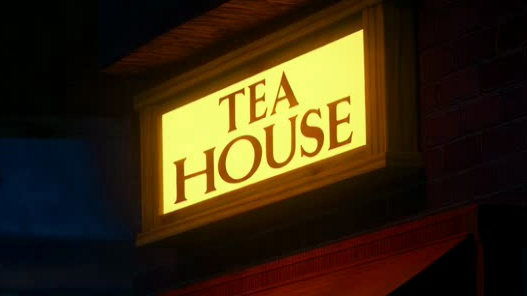
\includegraphics[width=0.27\linewidth]{figs/cells/fail_g058_en_signboard_s4_orig.jpg} & 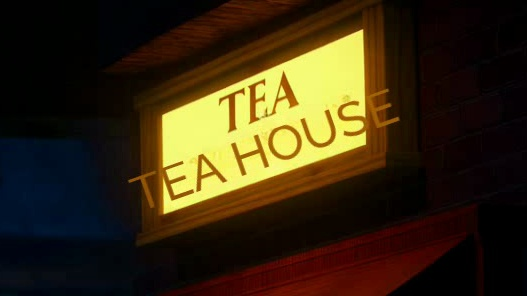
\includegraphics[width=0.27\linewidth]{figs/cells/fail_g058_en_signboard_s4_B1.jpg} & 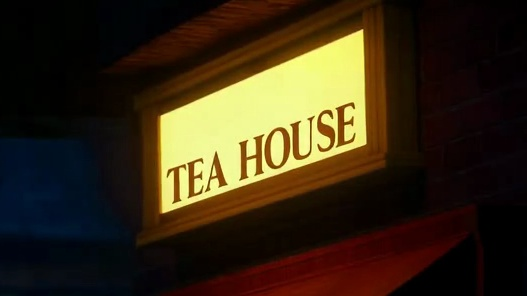
\includegraphics[width=0.27\linewidth]{figs/cells/fail_g058_en_signboard_s4_steervte.jpg} \\
&\parbox[t]{0.27\linewidth}{\centering\scriptsize \textcolor{okgreen}{\ding{51}}\,\texttt{TEA HOUSE}} & \parbox[t]{0.27\linewidth}{\centering\scriptsize \textcolor{badred}{\ding{55}}\,\texttt{TEA TEA HOUSE}} & \parbox[t]{0.27\linewidth}{\centering\scriptsize \textcolor{okgreen}{\ding{51}}\,\texttt{TEA HOUSE}} \\[3pt]
\scriptsize Neon glyph blurred & 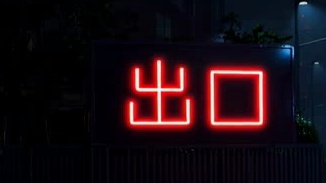
\includegraphics[width=0.27\linewidth]{figs/cells/fail_g076_zh_neon_s7_orig.jpg} & 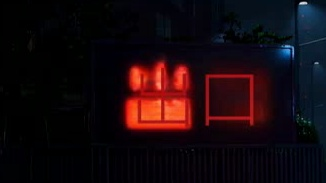
\includegraphics[width=0.27\linewidth]{figs/cells/fail_g076_zh_neon_s7_B1.jpg} & 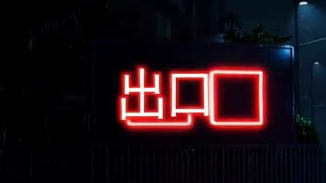
\includegraphics[width=0.27\linewidth]{figs/cells/fail_g076_zh_neon_s7_steervte.jpg} \\
&\parbox[t]{0.27\linewidth}{\centering\scriptsize \textcolor{okgreen}{\ding{51}}\,\texttt{\zh{出口}}} & \parbox[t]{0.27\linewidth}{\centering\scriptsize \textcolor{badred}{\ding{55}}\,\texttt{\zh{备份}}} & \parbox[t]{0.27\linewidth}{\centering\scriptsize \textcolor{okgreen}{\ding{51}}\,\texttt{\zh{出口}}} \\[3pt]
\end{tabular}
\caption{\textbf{Failure modes of Banksy} (hand-picked to cover each type; SteerVTE shown for reference). The first three keep the target readable but degrade appearance; the last three come from clips whose original was already correct and that Banksy broke.}
\label{fig:fail}
\end{figure*}


\subsection{Where \method fails}
\label{sec:failures}
\paragraph{Breaking correct text.} \method breaks \rOursBroken{} of the \rOrigCorrect{} originally correct clips (\steer: \rSteerBroken). In all of them, the evaluation reader transcribes the original correctly while the pipeline's OCR reads it correctly in at most 2\% of the frames (neon italics, extruded or condensed letters), so the preservation gate cannot fire. Inspecting the outputs (\cref{fig:fail}, last three rows) gives four failure types: new text larger than its sign, so that letters fall off the carrier (4 clips); old text left visible next to the new text, because a second row was not detected or the erasure was incomplete (5); wrong colour or contrast on lightboxes and extruded letters (2); and stacked two-row text on an LED screen that is still misread (1). In one of these clips the reader's verdict on the original is itself doubtful: the original shows a garbled four-character string, which the reader transcribes as \zh{电影院} in every frame.

\paragraph{Readable but not faithful.} The more common failure does not affect readability (\cref{fig:fail}, first three rows): erasure leaves a visible patch, or the new glyphs are flat where the old ones were outlined, extruded or glowing. These cases are frequent in the random sample of \cref{fig:qual} and explain the appearance distance in \cref{tab:main}.

\subsection{The appearance gap to generative editing}
\label{sec:limits}
Among the \rBothRepairN{} garbled clips that both methods repair, \steer's text is closer to the original appearance in \rSteerCloserPct\% (median appearance distance \rBothRepairMedSteer{} vs.\ \rBothRepairMedOurs), so the gap is not an artefact of \steer leaving garbled text untouched. We see four causes, in decreasing order of visibility.
\begin{itemize}
\item \textbf{Rendering instead of generation.} \method can reproduce colour, shading and, with SAT, glow; it cannot reproduce extrusion, bevels, tube geometry or texture inside the strokes, which a generator synthesises naturally.
\item \textbf{A small font library.} The library holds 33 Latin and 8 Chinese families, and the generator's typefaces are invented. In practice, \rLatinFam{} Latin families are selected, but for Chinese only \rZhFam, and Noto Sans SC alone renders \rNotoPct\% of the edited Chinese clips; the result reads correctly but looks uniform. Choosing the font by the shapes of the identifiable source letters (\cref{sec:exp_neg}) changed the font in only \rFshapeN{} clips.
\item \textbf{Axis-aligned layout.} The letter band inherits the orientation of the OCR quad, which is axis-aligned for most detectors, so on tilted carriers the new text can look skewed relative to the sign (\cref{fig:teaser}a); the perspective estimate of an earlier front end was too fragile to keep (supplement), and laying the text along the source baseline (\cref{sec:exp_neg}) could not be shown to help with our appearance metric, which does not see orientation.
\item \textbf{Erasure traces.} LaMa fills the hole once per clip; on textured or shaded carriers the fill is visible as a patch.
\end{itemize}
Two observations suggest that the gap is closable without giving up correctness. First, the garbled source already contains most of the target's characters: in garbled English clips, a median of \rCharsEn\% of the target letters occur in the reader's transcription of the original (Chinese: \rCharsZh\%). Reusing these glyphs---with their own font, colour, lighting and perspective---and synthesising only the missing ones would extend the ``change only what is wrong'' principle from words to characters; our first implementation (\cref{sec:exp_neg}) shows that the bottleneck is reliable letter segmentation and matching, which currently admits too few clips. Second, the two methods fail on different clips: the share of clips that at least one of them repairs is \rAtLeastOne\%. A combination that accepts a generative edit only when independent OCR verifies it, and otherwise falls back to deterministic repair, is a natural next step; its verifier must be strict, since accepting a wrong edit costs correctness, whereas rejecting a right one costs only appearance.

\subsection{Other limitations}
The benchmark is generated by one family of models and its prompts ask for short sign texts; a second generator (CogVideoX-5B, 360 clips from the same prompts) is part of our plan but has not been evaluated yet, and long texts such as menus or user interfaces are out of scope. Readability is measured by a VLM reader; it favours large, high-contrast text, which may flatter rendered glyphs, and it can transcribe a garbled original as the intended word (\cref{sec:failures}). A pre-registered second reader from another model family confirms the advantage over \steer, with a smaller margin that is significant for Chinese but not for English alone, and a third reader limited to English finds the methods level once its invented additions are discounted (\cref{sec:main}); readability claims therefore depend on the reader, and we report all of them. The appearance distance is glyph-agnostic and has a test--retest noise of \rRetestSD{} per clip (\cref{sec:exp_neg}): it supports large differences such as the gap to \steer and the effect of SAT, but not small ones. The human study on SAT used four raters after quality control; a registered blind comparison of \method with \steer on material naturalness, artifacts and temporal stability was not conducted for lack of raters, so the appearance comparison with \steer rests on the appearance distance and on visual examples. Finally, the preservation gate is safe but has low recall, because it relies on a conventional OCR that rarely reads stylised originals. Outside repair, on editing correct text (VTE-Bench), the frozen system is clearly behind \steer (\xVteOurs\% vs.\ \xVteSteer\%, \cref{sec:exp_external}), partly because its front end fails to locate \xVteFails{} of the 100 source texts.
